\documentclass[a4paper,english]{lipics-v2019}
\usepackage{microtype,amssymb,amsmath,stmaryrd,mathpartir,array,graphicx,tabularx}%if unwanted, comment out or use option "draft"
\usepackage[table]{xcolor}
\newcommand{\xt}[1]{\texttt{#1}}
%\newcommand{\tupleo}[1]{\xt{Tuple1\{}#1\xt{\}}}
\newcommand{\tuplet}[2]{\xt{Tuple\{}#1,#2\xt{\}}}
\newcommand{\union}[2]{\xt{Union\{}#1,#2\xt{\}}}
\newcommand{\denotes}[1]{\llbracket #1 \rrbracket}

%FZ
\newcommand{\sub}{<:}
\newcommand{\tuple}[1]{\xt{Tuple\{}#1\xt{\}}}
\newcommand{\arrayt}[1]{\xt{Array\{}#1\xt{\}}}
\newcommand{\FZ}[1]{\textbf{FZ says: #1}}
%end FZ

\newcommand{\goodcell}{\cellcolor{green!25}}
\newcommand{\badcell}{\cellcolor{red!25}}
\bibliographystyle{plainurl}% the recommnded bibstyle
\title{Julia's efficient algorithm for subtyping unions and covariant tuples}
\titlerunning{Subtyping union types and covariant tuples}

\author{Benjamin Chung}{Northeastern University}{}{}{}%mandato
\author{Francesco Zappa Nardelli}{INRIA}{}{}{}
\author{Jan Vitek}{Northeastern University \& Czech Technical University}{}{}{}

\authorrunning{B. Chung, F. Zappa Nardelli, J. Vitek}

\Copyright{Anon}%Benjamin Chung, Francesco Zappa Nardelli, Jan Vitek}%mandatory, plea
\ccsdesc[500]{Theory of computation~Type theory}
% mandatory: Please choose ACM 2012 classifications from https://www.acm.org/publications/class-2012 or https://dl.acm.org/ccs/ccs_flat.cfm . E.g., cite as "General and reference $\rightarrow$ General literature" or \ccsdesc[100]{General and reference~General literature}. 

\keywords{Type systems, Subtyping, Union types}

\category{}%optional, e.g. invited paper

\relatedversion{}%optional, e.g. full version hosted on arXiv, HAL, or other respository/website

\supplement{}%optional, e.g. related research data, source code, ... hosted on a repository like zenodo, figshare, GitHub, ...

\hideLIPIcs

\funding{}%optional, to capture a funding statement, which applies to all authors. Please enter author specific funding statements as fifth argument of the \author macro.

% jan comments 4/24/19
% code bits are fairly wordy; see if both OCaml and Coq can be trimmed down
% how clear are the code bits? 
% clarify last_left_to_right; do with a fold? <- attempted fix
% better motivate this in the intro
%    bit of julia? <- attempted fix
%    other features that make this important to solve? <- attempted fix
%    intro should be longer and take more time
% talks about semantic subtyping as if it's a fact, but doesn't explain what it is or why we should care <- attempted fix
% figures
%   haven't spent enough time looking at them
%   may not help
% references
%    subtyping cites
%       if there's one that's subsuming others then cite that
%       but if there's some alternatives then cite the lot



\acknowledgements{}%optional
%\acknowledgements{Celeste Hollenbeck}

%Editor-only macros:: begin (do not touch as author)%%%%%%%%%%%%%%%%%%%%%%%%%%%%%%%%%%
\EventEditors{John Q. Open and Joan R. Access}
\EventNoEds{2}
\EventLongTitle{42nd Conference on Very Important Topics (CVIT 2016)}
\EventShortTitle{CVIT 2016}
\EventAcronym{CVIT}
\EventYear{2016}
\EventDate{December 24--27, 2016}
\EventLocation{Little Whinging, United Kingdom}
\EventLogo{}
\SeriesVolume{42}
\ArticleNo{23}
%\nolinenumbers %uncomment to disable line numbering
%\hideLIPIcs  %uncomment to remove references to LIPIcs series (logo, DOI, ...), e.g. when preparing a pre-final version to be uploaded to arXiv or another public repository
%%%%%%%%%%%%%%%%%%%%%%%%%%%%%%%%%%%%%%%%%%%%%%%%%%%%%%

\begin{document}

\maketitle
\begin{abstract}
  We describe the algorithm implemented in the Julia
  programming language runtime to decide subtyping on a simple type
  system with union types, covariant tuples, and literals.  This
  algorithm is immune from the space-explosion and expressiveness
  problems of standard algorithms that normalise types into
  disjunctive normal form ahead-of-time.  We prove this algorithm
  correct and complete against a semantic-subtyping denotational model
  in Coq.
\end{abstract}

\section{Subtyping union types and covariant tuples}

Union types, originally introduced by Barbanera and Dezani-
Ciancaglini~\cite{barbanera1991intersection}, are increasingly common in
mainstream languages. In some cases, as Julia~\cite{BezansonEKS17} or
TypeScript~\cite{typescript}, they are exposed at the source level. In others,
such as Hack~\cite{hack}, they are only used internally when performing type
inference. In all cases, they play a key role in the expressiveness of the
language.

Rules for subtyping union types have been known for a long time.  Following Vouillon~\cite{Vouillon04} they may be written as:
\begin{mathpar}
\inferrule{t_1 \sub t \\ t_2 \sub t}{\union{t_1}{t_2} \sub t}

\quad

\inferrule{t \sub t_1}{t \sub \union{t_1}{t_2}}

\inferrule{t \sub t_2}{t \sub \union{t_1}{t_2}}
\end{mathpar}
These rules are asymmetrical. Following from set-theoretic intuitions,
and as made formal by semantic subtyping models, when a union type
appears on the left-hand side of a subtype judgment, then \emph{all}
its components must be subtypes of the right-hand side; whan a union
type appears on the right-hand side of a subtype judgment, then there
must \emph{exist} a component that is a supertype of the
left-hand side.

While this rule system makes sense, it leads to some surprising results.
The notion that subtyping should allow the substitution of any subtype
for a supertype is both natural and common. Under this justification, 
one might logically expect a union type to act as a set-theoretic union. 
However, with a trivial addition to our type language the above rules 
violate the set-theoretic underpinning that would be expected from a 
semantic subtyping~\cite{Pierce1991} system.

Let us recall the subtype rule for covariant tuples:
\[
\inferrule{t_1 \sub t'_1 \\ t_2 \sub t'_2}{\tuple{t_1, t_2} \sub \tuple{t'_1, t'_2}}
\]
When we add this rule to our system, unusual behaviour then appears. Consider
the following judgment:
\[
\tuple{\union{t_1}{t_2}, t} \ \ \sub\ \ \union{\tuple{t_1, t}}{\tuple{t_2, t}} 
\]
If we were to assume a semantic semantics for our type system, this judgment should
hold. The left hand side denotes the values $\{\tuple{v_1,v_2}\} | v_1 \in \llbracket t_1 \rrbracket \cup \llbracket t_2 \rrbracket \wedge v_2 \in \llbracket t \rrbracket \}$,
and the right hand side denotes $\llbracket \tuple{t_1, t} \rrbracket \cup \llbracket \tuple{t_2, t} \rrbracket$, where $\llbracket t \rrbracket$ indicates the
set of values denoted by $t$. It is obvious that these two sets are the same, and thus under
a semantic understanding of subtyping we would therefore conclude that our judgment should be 
derivable.

However, under the above proposed rules for subtyping of unions and tuples the
subtyping relation cannot be concluded. Under the above rules, we must pick a
choice of the  right-hand union to continue. However, any choice we make will
cause the right-hand-side to become overspecialized; picking the left or right
choices at the union will cause the right-hand-side to match $t_1$ or $t_2$ in 
the first position, yet the left-hand-side could take on \emph{either} in that 
position.

The standard  approach to solve this conundrum is to \emph{rewrite all types
into their disjunctive normal form} (DNF), as unions of union-free types,
\emph{before} building the derivation. The correctness of this rewriting step
is justified by the semantic-subtyping denotational model, as
in~\cite{Frisch08}, and the resulting subtype algorithm can be proved both
correct and complete.  However, this standard algorithm based on ahead-of-time
normalization has \emph{two major drawbacks}.

The first drawback is that the normalization phase rewrites types into
potentially \emph{exponentially bigger} types, a serious practical problem.
The Julia programming language allows programmers to write union types in function
arguments, types that must then be compared against actual types at call sites using
subtyping. Previous work~\cite{DBLP:NardelliBPCBV18} instrumented Julia's subtype
decision procedure to examine the prevalance and use of such union types, and routinely observed queries
such as the following:

\begin{small}
\begin{verbatim}
 Tuple{Tuple{Union{Int64, Bool}, Union{String, Bool}, Union{String, Bool}, 
             Union{String, Bool}, Union{Int64, Bool}, Union{String, Bool}, 
             Union{String, Bool}, Union{String, Bool}, Union{String, Bool}, 
             Union{String, Bool}, Union{String, Bool}, Union{String, Bool}, 
             Union{String, Bool}, Union{String, Bool}, Union{String, Bool}}, Int64}
\end{verbatim}
\end{small}
Normalizing this type before attempting to decide subtyping is not a
realistic option. Each choice at each union can be thought of as a digit in a
binary number, all of which must be expanded when normalizing, so the 
fully-normalized form would have $2^15$ or 32,768 terms. Storing this normalized
type is not practical.

Moreover, full expansion is frequently unnecessary. In practice, such types are often 
matched against structurally simpler types like
\begin{small}
\begin{verbatim}
 Tuple{Tuple{Any, Any, Any, Any, Any, Any, Any, Any, Any, Any, Any, Any, Any, Any, Any}, 
       Any}
\end{verbatim}
\end{small}
(where in Julia \verb+Any+ is the supertype of all types). If we forgo
normalisation, it is possible to decide subtyping with such simple types
in linear time. This performance would be vastly preferred to the exponential
time performance of normalisation.

The second drawback of the ahead-of-time normalisation phase is that it
does not interact well with other type system features. For instance,
\emph{invariant constructors} make lifting all union types to the top
level unsound.
Consider the type \(\arrayt{\union{t_1}{t_2}}\), where \texttt{Array}
is an invariant unary constructor.  This type
denotes the set of arrays whose elements are either of type \(t_1\) or
\(t_2\); it would be incorrect to rewrite it as
\(\union{\arrayt{t_1}}{\arrayt{t_2}}\),
as this latter type denotes the set of arrays
whose elements are either all of type \(t_1\) or all of type
\(t_2\).  A weaker disjunctive normal form, only lifting union types inside
each invariant constructor, can circumvent this
problem. However, doing so only to reveals a deeper problem in the presence of
 both invariant constructors and \emph{existential types}.
Consider the judgment below:
\[
  \arrayt{\union{\tuple{t_1}}{\tuple{t_2}}} \ \ <:\ \ \exists T\,.\, \arrayt{\tuple{T}}
\]
This judgment holds by taking \(T = \union{t_1}{t_2}\).  Since all
types are in weak normal form, a standard algorithm would initially
perform the left-to-right subtype check due to the outer invariant
constructor.  This step would generate the constraint \(T >:
\union{t_1}{t_2}\).  As a consequence, the subsequent right-to-left
check due to the invariant constructor fails.  Indeed this requires
proving that \(\tuple{T} <: \union{\tuple{t_1}}{\tuple{t_2}}\), which
in turns attempts to prove either \(T <: t_1\) or \(T <: t_2\),
both unprovable under the assumption that \(T >: \union{t_1}{t_2}\)
The key to derive a successful judgment for this relation is to rewrite the
right-to-left check into \(\tuple{T} <: \tuple{\union{t_1}{t_2}}\),
which is provable. This is a sort of \emph{anti-normalisation} rewriting that
must be performed on sub-judgments of the derivation, and to the best
of our knowledge it is not part
of any subtype algorithm based on ahead-of-time disjunctive normalisation.

Previous work has either not offered distributivity or uses normalisation.
The earliest work, by Barbanera and Dezani-Ciancaglini~\cite{barbanera1991intersection} and
Pierce~\cite{Pierce1991} uses normalization to decide distributive subtyping between
union types. Vouillon~\cite{Vouillon04} does not support distributivity at all as a limitation 
of their approach. 


%% FZN : Duplicate of text already written
%% FZN : fix citations above though.
%%
%% Previous efforts to provide a decision procedure for distributive unions rely
%% heavily on normalization. In order to decide subtyping in one of these
%% approaches, the type is first normalized (to integrate the distributivity
%% axiom) and then the standard syntax-directed subtyping algorithm is applied to
%% conclude the subtyping
%% relation~\cite{muehlboeck2018empowering,Reynolds1997,Pierce1991}. This
%% normalization step puts the type into disjunctive normal form thereby allowing
%% the algorithmic union rule to decide subtyping correctly. As there are
%% exponentially many choice sets for any given type (where one of two choices
%% may be given at each union), the space taken up by the fully normalized type
%% can be substantial. Moreover, (in languages with some kind of higher-rank
%% polymorphism) the normalization process eliminates all internal unions; as a
%% concequence, variable instantiations may be over-specialized and some
%% semantically-valid subtyping relations may not hold.

In this \emph{pearl paper} we describe the keys ideas used by the
subtype algorithm implemented in the Julia language to deal with
union types and covariant tuples, and we will argue that these avoid the
two drawbacks above.  To avoid being drawn in the vast complexity of
Julia type algebra, we focus on a minimal language featuring union
types, covariant tuples, and literals.  This tiny language is
expressive enough to highlight the decision strategy, and make this
implementation technique known to a wider audience.  While Julia
implementation shows that this technique extends, among others, to
invariant constructors and existential
types~\cite{DBLP:NardelliBPCBV18}, we expect that it
can be leveraged in many other modern language designs.  Additionally
we prove in Coq that the algorithm is correct and complete with
respect to a standard semantic subtyping model.


\section{A space-efficient algorithm}

The greatest difficulty of subtyping union types is searching the entire space
of possible forall/exist quantifications of union types. We have seen that
syntax-directed rules need ahead-of-time normalisation in the presence of
covariant tuples.

The algorithm we propose for deciding subtyping works by iterating through
choices made at unions along paths complete through the two types In this
section, we will describe the implementation of the algorithm in OCaml and
will present our proof of correctness in Coq in the following section.

We focus on a core type language composed of binary unions, covariant binary
tuples, and atom types:
\begin{small}
\begin{verbatim}
  type typ =
    | Atom of int
    | Tuple of typ * typ
    | Union of typ * typ
\end{verbatim}
\end{small}
Atom types are singletons with respect to subtyping, and are ranged
over by
\(A, B, ...\).  Abusing the
notation, we will assume that we also have unary
tuples; these can be easily encoded. 

%% Begin structural iterator based description

We will begin by discussing a version of our algorithm that uses structurally-
dependent iterators to explore types, then use that basis to describe our
final space-efficient formulation and possible optimization thereof. 

The fundamental operation the algorithm must accomplish is deciding if
for every possible choice on the left if there exists some choice on the
right such that subtyping holds. In order to do this, the algorithm iterates
through each possible choice; both structural and space-efficient algorithms
iterate over the same types in the same order, but do so using different yet 
isomorphic internal representations.

A structural iterator can be thought of as a sub-tree of the overarching type
tree; we show these sub-trees in blue in figure~\ref{fig:cfs}. As there are no
tuples in this example, the sub-trees are in fact paths for this case. It can
be easily seen that we explore every path through the given type tree.

The main question is: "how do we step from one sub-tree to the next?" In order
to explore every sub-tree, our algorithm finds the deepest (top-to-bottom,
left-to-right) union where it took the left branch and generates a new tree
where it instead takes the right branch. This is seen in
figure~\ref{fig:sstep}, where the deepest union in the initial state is the
root; the algorithm flips this to take the right choice and then fills out the
sub-tree with left choices until it reaches a  leaf.

Storing sub-trees is expensive, however, as it requires storing a very incomplete
tree structure. Our space-efficient representation encodes the same information as 
the sub-trees, but does so without itself being aware of the type being iterated over's
structure. It linearizes the choices made to construct the sub-tree into a list, which
can then be manipulated in a manner isomorphic to the sub-trees.

Our space efficient representation stores choices that are made along a pre-order depth-first
traversal of the iterated type tree. We can then manipulate this representation directly, avoiding
the construction or storage of tree-structured iterators. The choices are stored as lists of 
\verb|st_choice|s which
indicate which branch of a union type was taken:
\begin{small}
\begin{verbatim}
  type st_choice = Left | Right
\end{verbatim}
\end{small}

Lists of \verb|st_choice|s are isomorphic to the sub-tree representation when
combined with the type being iterated over. To convert from sub-trees  to
choice lists we simply conduct a preorder traversal of the sub-tree recording
which choices were made along the way. Going from choice lists to sub-trees can
be done by traversing the full type using the choice list while adding the traversed
nodes to the sub-tree.

% The algorithm stores
% the choice made at each union at the present iteration in two stacks of
% \verb|st_choice|s, one for each side of the subtype relation. 
% Each \verb|st_choice| stack can be seen as the state of an iterator that
% enumerates every union-type induced alternative in a given type.  One
% stack will be used to ensure that all \emph{forall} choices have been
% explored; the other stack to search for a matching \emph{exist} choice.
% In figure~\ref{fig:cfs}, these are depicted as the $\forall$ and $\exists$ stacks.

% It is possible to define both an initial element and next state function for
% iterators defined using \verb|st_choice| stacks.

Since our algorithm moves left-to-right through the type tree, we will
initialize it with the state that takes the left choice at every union:

\begin{small}
\begin{verbatim}
  let rec initial_choice (a:typ) = 
    match a with
    | Atom i -> []
    | Tuple(t1,t2) -> (initial_choice t1) @ (initial_choice t2)
    | Union(l,r) -> Left::(initial_choice l)
\end{verbatim}
\end{small}
%  | Tuple1 t -> initial_choice t

\begin{figure}
\centering
\begin{tabularx}{\linewidth}{c|ccc}
& Initial & Stepped & Padded\\
Subtree: &
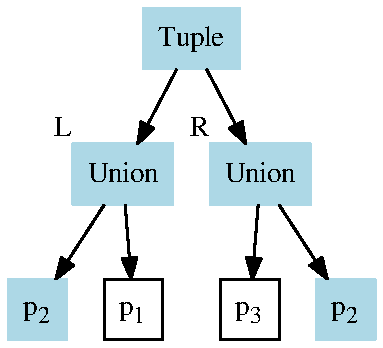
\includegraphics[scale=0.55]{figures-gen/transex1.pdf} & 
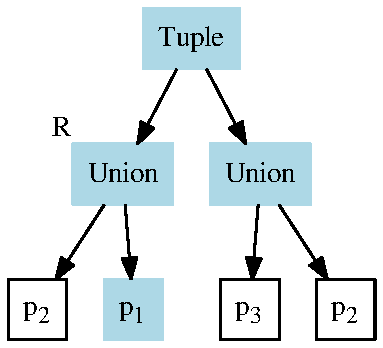
\includegraphics[scale=0.55]{figures-gen/transex2.pdf} & 
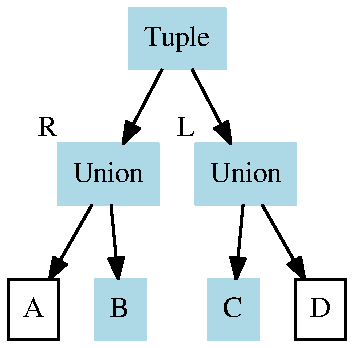
\includegraphics[scale=0.55]{figures-gen/transex3.pdf} \\
Choice List: & \underline{L}R & \underline{R} & \underline{R}L \\
Effective Type: & \tuple{A,D} & \tuple{B,?} & \tuple{B,C} \\
\end{tabularx}
\caption{State-stepping operation for choice lists}
\label{fig:sstep}
\end{figure}

Next, we define the step function. In the sub-tree intuition, we want to find
the deepest union (left-to-right through tuples) in our current sub-tree where
we made a left choice. In our resulting sub-tree, we take the alternative
(right) choice at this deepest left choice, then make left choices until we
reach a leaf. This operation is visualized in figure~\ref{fig:sstep}. The next
state is defined as the one where we take the right choice at the deepest left-to-right
left choice, then complete the sub-tree with left choices. To implement this,
we can describe the operation in two steps: stepping and padding.

When stepping, we identify the deepest left-to-right left choice and make it
into a right then get rid of all following choices. In the sub-tree, we do
this by simply working through the sub-tree from bottom-to-top, right-to-left
until we find a choice where we went left and making that into a right. The
following choices are then dropped from the sub-tree. The result of this is
shown as the stepped subtree in figure~\ref{fig:sstep}.

We can define an equivalent operation over choice lists. Since choice lists
can be constructed from a sub-tree by iterating through them depth-first left-
to-right, the bottom-to-top right-to-left search for a left choice in the
subtree is equivalent to finding the \emph{last} left choice in the choice
list. This choice is turned into a right and the remainder of the list is then
truncated.

To implement this, we first reverse the choice list, replace the first left
in the reversed list with a right choice, and then throw away the choices that
we've encountered in the reversed list so far. We then reverse the result to
produce the new choice list in correct order. This is implemented in the
\verb|last_left_to_right| function, shown below.

\begin{small}
\begin{verbatim}
let rec toggle_truncate = function
  | [] -> []    
  | Left::tl -> Right::tl
  | Right::tl -> toggle_truncate tl

let last_left_to_right (l:st_choice list) =
  match List.rev (toggle_truncate (List.rev l)) with
  | [] -> None
  | hd::tl -> Some(hd::tl)
\end{verbatim}
\end{small}

The stepped state is incomplete, however. The first element of the tuple has now
changed, but the second element is no longer defined by either the sub-tree or its
equivalent choice list. In order to define this second element, we need to complete
the sub-tree and pad out the choice list. 

The padding operation, taking the stepped state and producing the padded one, is determined
by the direction of iteration. Since we go left-to-right through the type, we need to start
any new iteration with making all left choices. Therefore, when presented by stepping with
a partial sub-tree or choice list, we will pad it out with left choices until we have a complete
tree or choice list.

We show the padding operation for choice lists in OCaml, named
\verb|extend_list|, below.  The correct padding is computed recursively from
the type being iterated through by following the given choice list until it
runs out, then adding lefts until all branches have been explored.

\begin{small}
\begin{verbatim}
  let rec extend_list (a:typ) (ls:st_choice list) = match (a,ls) with
    | (Atom i, _) -> ([], ls)
    | (Tuple(t1,t2), _) -> let (hd,tl) = extend_list t1 ls in
                           let (hd2,tl2) = extend_list t2 tl in
                           (hd @ hd2, tl2)
    | (Union(l,r), Left::rs) -> let (hd,tl) = extend_list l rs in (Left::hd,tl)
    | (Union(l,r), Right::rs) -> let (hd,tl) = extend_list r rs in (Right::hd,tl)
    | (Union(l,r), []) -> (Left::initial_choice l,[])
\end{verbatim}
\end{small}


Finally, the \verb|next_state| function combines these operations into
a single step operation. It will take the deepest alternative choice
at a union using \verb|last_left_to_right|, then add however many left
choices are required to make the path valid using \verb|extend_list|. The
complete \verb|next_state| operation shown in figure~\ref{fig:sstep} takes
the choice stack L and the type $\union{A}{\union{B}{C}}$ and produces the
choice stack RL. To do so, it takes the left choice, converts it to a right,
then pads the list out with lefts until the path is valid with respect to the 
type.
\begin{small}
\begin{verbatim}
  let rec next_state (a:typ) (ls:st_choice list) =
    option_map fst (option_map (extend_list a) (last_left_to_right ls))
\end{verbatim}
\end{small}

\subsection{Subtyping}

\begin{figure}[h]
\center
\begin{tabular}{cc|cc|c}
\multicolumn{2}{c}{Stack} & \multicolumn{2}{c}{Type} & Base Query \\
\hline
$\forall$ & $\exists$ & $\forall$ & $\exists$ & \\
\hline
\goodcell L & \goodcell L & \goodcell 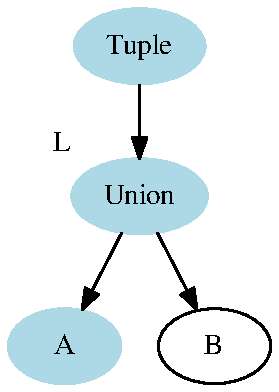
\includegraphics[scale=0.3]{figures-gen/left1.pdf} & \goodcell 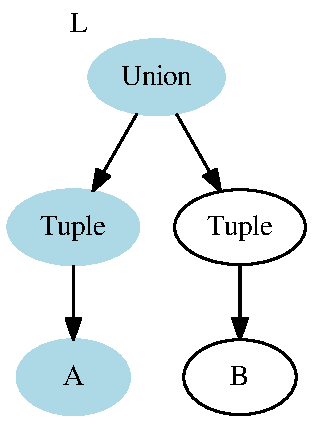
\includegraphics[scale=0.3]{figures-gen/right1.pdf} 
    & \goodcell ${A} <: {A}$ \\
\goodcell L & \badcell R & \badcell 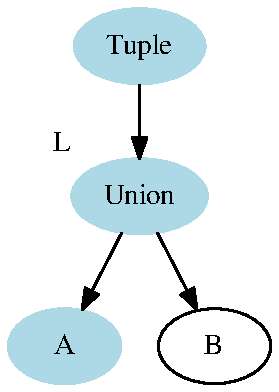
\includegraphics[scale=0.3]{figures-gen/left1.pdf} & \badcell 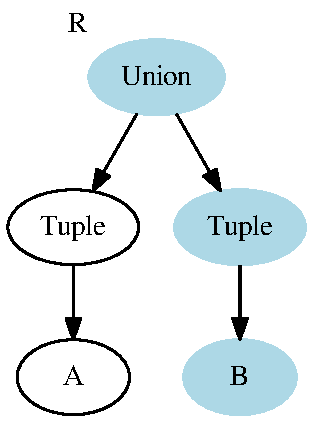
\includegraphics[scale=0.3]{figures-gen/right2.pdf}  
    & \badcell ${A} \not<: {B}$ \\
\hline
\goodcell R & \badcell L & \badcell 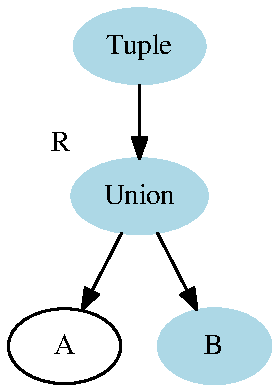
\includegraphics[scale=0.3]{figures-gen/left2.pdf} & \badcell 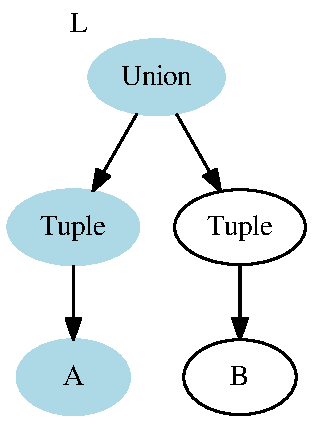
\includegraphics[scale=0.3]{figures-gen/right1.pdf}  
    & \badcell ${B} \not<: {A}$ \\
\goodcell R & \goodcell R & \goodcell 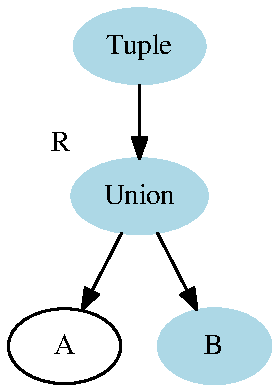
\includegraphics[scale=0.3]{figures-gen/left2.pdf} & \goodcell 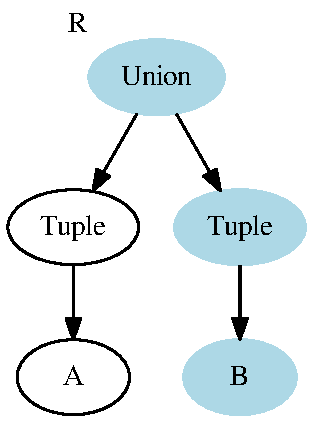
\includegraphics[scale=0.3]{figures-gen/right2.pdf}  
    & \goodcell ${B} <: {B}$ \\
\hline
\end{tabular}

\hspace{1em}

$\tuple{\union{A}{B}} <: \union{\tuple{A}}{\tuple{B}}$

\caption{Subtyping decision procedure example}
\label{fig:cfs}
\end{figure}

Now that we have defined the core iterator infrastructure, we show how it
is used to decide subtyping queries. Subtyping is defined on a forall-exists
basis, or for every choice on the left there must exist a choice on the right
such that basic subtyping (in our case, subtyping without unions) holds. We
use our iterator framework to implement this in the straightforward manner, 
iterating through each choice on each side and checking if a relationship holds.

To illustrate our algorithm, we use the  distributivity example from the
introduction: $$\tuple{\union{A}{B}} <: \union{\tuple{A}}{\tuple{B}}$$
Figure~\ref{fig:cfs} shows our algorithm's internal state when using  both the
structural and space- efficient representations when deciding subtyping for
this type.

The algorithm proceeds by maintaining two iterators (one for each side of the subtyping judgment) over choices-at-unions,  
checking that for every instantiation of the left hand type there
exists an instantiation of the right hand type. We will first define the
fundamental subtyping relation, used to decide subtyping relationships when
given instantiations of the left and right hand types, then describe the
algorithm that iterates through those types.

\begin{small}
\begin{verbatim}
  type st_res =
    | Subtype of st_choice list * st_choice list
    | NotSubtype
\end{verbatim}
\end{small}

The type \verb|st_res| represents the results of a single base subtype query. The query
can either succeed, in which case it provides the unused portion of the input
stacks, or fail. 

\begin{small}
\begin{verbatim}
  let rec base_subtype (a:typ) (b:typ) (fa:st_choice list) (ex : st_choice list)
    match (a,b,fa,ex) with
    | (Atom i, Atom j, _, _) -> if i == j then Subtype(fa, ex) else NotSubtype
    | (Tuple(ta1, ta2), Tuple(tb1, tb2), _, _) ->
       (match base_subtype ta1 tb1 fa ex with
        | Subtype(cfa, cex) -> base_subtype ta2 tb2 cfa cex
        | NotSubtype -> NotSubtype)
    | (Union(a1,a2),b,choice::fa,ex) -> 
                base_subtype (match choice with Left -> a1 | Right -> a2) b fa ex
    | (a,Union(b1,b2),fa,choice::ex) -> 
                base_subtype a (match choice with Left -> b1 | Right -> b2) fa ex
\end{verbatim}
\end{small}

The function \verb|base_subtype| is responsible for using two
paths---one for the left and right hand sides of the subtyping
relation---and checking that the subtype relation holds with respect
to those paths. Given a basic type---an atom or a tuple---it will
either check equality or recur respectively. Given a union type, it
will choose the component of the union type following the choice
stacks and continue recursively. The function then returns an instance
of \verb|st_res|, which gives the remaining choice stacks if
successful or nothing otherwise.

\par
Finally, to check subtyping, we need to iterate through both types in the 
correct quantification order. Subtyping holds if, for every instantiation 
of the left there exists an instantiation of the right hand side of the
subtyping judgment such that the subtype relation holds. To check this,
we use a simple brute force approach sitting atop the choice stack iterator
infrastructure described previously. The algorithm is implemented in two
functions. \verb|ex_subtype| checks that there exists an instantiation
of the right-hand-side for a given left-hand-side. \verb|fa_ex_subtype|
uses \verb|ex_subtype| to check that for every instantiation of the LHS,
there is an instantiation of the RHS such that the subtype relation
holds. 
\par
\begin{small}
\begin{verbatim}
  let rec ex_subtype (a:typ)(b:typ)(fa:st_choice list)(cex : st_choice list) =
    match base_subtype a b fa cex with (* is a <: b *)
    | Subtype(_,_) -> true (* there exists a subtype *)
    | NotSubtype -> 
       (match next_state b cex with (* step exists-env *)
        | Some ns -> ex_subtype a b fa ns (* continue *)
        | None -> false) (* no subtype; exit *)
\end{verbatim}
\end{small}
If the current choice---given by \verb|cex|---is a supertype of the given \verb|a| according
to \verb|base_subtype|, then \verb|ex_subtype| has found a valid instantiation of \verb|b|. Therefore,
there exists an instantiation of \verb|b| that is a supertype of \verb|a| and the result should be true.
Otherwise, \verb|ex_subtype| will use the iteration operation, \verb|next_state|, to continue iterating
through choices for \verb|b| until it either finds an instantiation that is a supertype or runs out
of instantiations.

\begin{small}
  \begin{verbatim}
  let rec fa_ex_subtype (a:typ)(b:typ)(cfa:st_choice list) =
    match ex_subtype a b cfa (initial_choice b) with (* a <: b wrt path? *)
    | true -> (match next_state a cfa with
               | Some ns -> fa_ex_subtype a b ns (* continue *)
               | None -> true) (* all subtypes; is subtype *)
    | false -> false (* exists a non-subtype; not subtype *)
\end{verbatim}
\end{small}

The function \verb|fa_ex_subtype| is similar; it checks that for every
instantiation of \verb|a|, there exists an instantiation of 
\verb|b| such that subtyping holds. Checking for an instantiation
of \verb|b| is done using \verb|ex_subtype|, while \verb|fa_ex_subtype|
maintains an iterator for \verb|a|.

The operation of \verb|fa_ex_subtype| and \verb|ex_subtype| as well as their
calls to \verb|base_subtype| can be seen in figure~\ref{fig:cfs}. In the
$\forall$ column, we see the current state maintained by \verb|fa_ex_subtype|.
The $\exists$ column shows the state maintained by \verb|ex_subtype| as it is
called by \verb|fa_ex_subtype|. In the example, for a forall-list of L, we an
find an exists-list of L such that \verb|base_subtype| holds. Similarly,
for a forall-list of R, we can find an exists-list instantiation of R such
that subtyping holds. Therefore, for every instantaition of the left-hand-side,
there exists an instantiation of the right-hand-side such that subtyping holds
and subtyping holds for the type as a whole.


\begin{small}
\begin{verbatim}
  let subtype (a:typ) (b:typ) = fa_ex_subtype a b (initial_choice a)
\end{verbatim}
\end{small}

Finally, \verb|subtype| checks if \verb|a| is a subtype of \verb|b|.
It seeds \verb|fa_ex_subtype| with the initial choice for \verb|a|'s
iterator, which then checks if for every instantiation of \verb|a|
there exists an instantiation of \verb|b| such that subtyping holds.

We have presented our subtyping algorithm using lists of choices. In a
practical implementation, however, these lists of choices can be efficiently
implemented (without allocation) by means of bit sets. This is the approach
taken in the Julia implementation of this algorithm. With this optimization,
the needed memory to decide a subtyping judgment is linear in the total number
of unions in the given types; the algorithm needs no allocation beyond that
of the choice stacks themselves.

\section{Correctness and completeness}

To prove correctness of our algorithm, we begin by formally specifying
correctness for subtyping. We then show that two subtyping algorithms---
based on structural iterators and choice lists---are correct
with respect to this definition in Coq.

We base our definition of subtyping on a denotational semantics for types. 
We reduce types in the type language including unions to sets of types
in the type language without unions through a simple transformation. 

\begin{align*}
\denotes{\xt{A}} &= \{A\} \\
\denotes{\union{t_1}{t_2}} &= \denotes{t1} \cup \denotes{t2} \\
\denotes{\tuplet{t_1}{t_2}} &= \{\tuplet{t'_1}{t'_2} | t_1' \in \denotes{t_1},  t_2' \in \denotes{t_2'}\} \\
\end{align*}

Using this denotational semantics for types-with-unions, we can define
subtyping as if $\denotes{t_1} \subseteq \denotes{t_2}$, then $t_1 <: t_2$.
Equivalently, we can state this as definition~\ref{dfn:scr}, which is canonicalized
in our Coq proof as the \verb|NormalSubtype| relation.

\begin{definition}[Subtyping Correctness]
A subtyping relation $<:$ is correct if $t_1 <: t_2$ iff $\forall t_1' \in \denotes{t_1},
\exists t_2' \in \denotes{t_2}, t_1 <: t_2$.
\label{dfn:scr}
\end{definition}

Proving a subtyping algorithm sound and complete is therefore equivalent to
producing a function of type \verb|forall t1 t2:type, {NormalSubtype t1 t2} + {~NormalSubtype t1 t2}|; that is, is able to decide whether two types are
subtypes or not.

We will begin by describing and proving correct a version of the algorithm
that uses explicit type-structural iterators. We will then show the choice
stack-based algorithm correct by proving equivalence between structural
iterators and choice stacks. In doing so, we will derive an induction
principle for structural iterators (and, as an extension, for choice stacks).

\subsection{Iterators}

The Coq iterator-based implementation is directly equivalent (as will be shown
later) to the choice-stack based implementation presented previously in OCaml.
However, it retains type structure information inside of the iterator state.

\begin{small}\begin{verbatim}
Inductive TypeIterator: type -> Set :=
| TIAtom : forall i, TypeIterator (atom i)
| TITuple : forall t1 t2, TypeIterator t1 -> TypeIterator t2 -> TypeIterator (tuple t1 t2)
| TIUnionL : forall t1 t2, TypeIterator t1 -> TypeIterator (union t1 t2)
| TIUnionR : forall t1 t2, TypeIterator t2 -> TypeIterator (union t1 t2).
\end{verbatim}\end{small}

The \verb|TypeIterator| structure follows the structure of the type being
iterated over. Choices at unions are represented as either an instance of
\verb|TIUnionR| or \verb|TIUnionL|. This structure then lets us trivially
define a function that extracts the current type at the iterator's position:

\begin{small}\begin{verbatim}
Fixpoint current (t:type)(ti:TypeIterator t):type :=
match ti with
| TIAtom i => atom i
| TITuple ti1 ti2 p1 p2 => tuple (current ti1 p1) (current ti2 p2)
| TIUnionL ti1 ti2 pl => (current ti1 pl)
| TIUnionR ti1 ti2 pr => (current ti2 pr)
end.
\end{verbatim}
\end{small}

\noindent We can then define a function that produces the initial iterator state for a
given type:

\begin{small}
\begin{verbatim}
Fixpoint start_iterator (t:type):TypeIterator t :=
  match t with
  | (atom i) => TIAtom i
  | (tuple t1 t2) => TITuple t1 t2 (start_iterator t1) (start_iterator t2)
  | (union t1 t2) => TIUnionL t1 t2 (start_iterator t1)
  end.
\end{verbatim}
\end{small}

\noindent Next, we can define a step function that takes one state and either steps it
to the next state or indicates that no such next state exists.

\begin{small}\begin{verbatim}
Fixpoint next_state (t:type)(ti:TypeIterator t) : option (TypeIterator t) :=
  match ti with
  | TIAtom i => None
  | TITuple ti1 ti2 p1 p2 =>
    match (next_state ti2 p2) with
    | Some np2 => Some(TITuple ti1 ti2 p1 np2)
    | None =>
      match (next_state ti1 p1) with
      | Some np1 => Some(TITuple ti1 ti2 np1 (start_iterator ti2))
      | None => None
      end
    end
  | TIUnionL ti1 ti2 pl =>
    match (next_state ti1 pl) with
    | Some npl => Some(TIUnionL ti1 ti2 npl)
    | None => Some(TIUnionR ti1 ti2 (start_iterator ti2))
    end
  | TIUnionR ti1 ti2 pr => option_map (TIUnionR ti1 ti2) (next_state ti2 pr)
  end.
\end{verbatim}\end{small}

With these definitions, we can then prove a basic form of correctness with
respect to the denotational or normalization semantics:

\begin{theorem}[Correctness of iterators]\begin{verbatim}
Remaining t (start_iterator t) (clauses t)
\end{verbatim}
Every type in $\denotes{t}$ will be explored using \verb|next_step| from \verb|start_iterator t|. 
\end{theorem}
\begin{proof}
The \verb|Remaining| predicate relates iterators to the list of types that remain to be iterated, so
the Coq theorem statement indicates that the initial state of the iterator for type $t$ has every clause
in the normalized version of $t$ remaining to be iterated.

We proceed by induction on $t$. The cases for atomic types and unions follow
from the IH trivially. We prove the theorem for tuples correct by case analyzing
on the number of clauses induced by the first element in the tuple, then identifying
the next element produced by the iterator from the tuple.

See \verb|iterator_has_clauses| in the Coq proof for full details.
\end{proof}

\verb|next_state| returns \verb|Some s| if there is some successor state
\verb|s| to the current, and \verb|None| if the given iterator state is
terminal. It will go left-to-right through unions, and will explore 2-tuples
by iterating through the choices on the right for each choice on the left. We can
then define an induction principle for type iterators based on \verb|next_state|:

\begin{theorem}
\begin{small}\begin{verbatim}
Definition iter_rect
  (t:type) (P:TypeIterator t -> Set)
           (pi: forall it, next_state t it = None -> P it)
           (ps : forall it' it'', P it'' -> next_state t it' = Some it'' -> P it')
           (it : TypeIterator t) : P it  
\end{verbatim}\end{small}

For any type \verb|t| and proposition \verb|P|, and if:
\begin{itemize} 
	\item \verb|P| holds for an iterator that has no next state (e.g. is done)
	\item if \verb|P| holds for the \emph{following} iterator state \verb|it|,
	then \verb|P| holds for the \emph{preceeding} iterator state \verb|it'|.
\end{itemize}
Then \verb|P| holds for all iterators for type \verb|t|
\end{theorem}
\begin{proof}
Proving the induction principle for type iterators relies on the \verb|iternum|
function, which decides the number of steps remaining in the iterator before termination.
The proof proceeds by simultaneous case analysis on the number of remaining states and
whether the iterator step function can produce a successor state from the present state.

If the iteration number is not yet 0, and if there is a successor state, then
we simply  appeal to the induction hypothesis and continue on. If there is no
successor state but  the iteration number is nonzero or vice versa, then by
lemma (\verb|iternum_monotonic|, taking an iterator step decrements the
iteration number) contradiction. Finally, if there is no next step and the iteration
number is 0, then we have reached the base case and terminate.

For full details, see the Coq definition of \verb|iter_rect|.
\end{proof}

Using \verb|iter_rect|, we can implement and prove correct equivalent functions
to \verb|ex_subtype|, \verb|fa_ex_subtype|, and \verb|subtype| as described in the
OCaml implementation.

\begin{small}\begin{verbatim}
Definition exists_iter(a b : type) : 
  ({ t | InType t b /\ BaseSubtype a t } +
   {forall t, InType t b -> ~(BaseSubtype a t) }).
\end{verbatim}\end{small}

\verb|exists_iter| is equivalent to the choice-stack based \verb|ex_subtype|,
and determines if there exists some denotationally-contained type in \verb|b|
that is a supertype of the given \verb|a|. Internally, it is implemented in 
the same way as \verb|ex_subtype|, though using \verb|iter_rect| to iterate 
through every iterator state.

\begin{small}\begin{verbatim}
Definition forall_iter (a b : type) :
  { forall t, In t (clauses a) -> exists t', InType t' b /\ (BaseSubtype t t')} +
  { exists t, In t (clauses a) /\ forall t', InType t' b -> ~ (BaseSubtype t t')}.
\end{verbatim}\end{small}

\verb|forall_iter| is to \verb|fa_ex_subtype| what \verb|exists_iter| is to
\verb|ex_subtype|. Like \verb|exists_iter| it implements the same decision procedure
as \verb|fa_ex_subtype| (and internally relies upon \verb|exists_iter|), though through
the abstraction of \verb|iter_rect|.

Finally, we can define a decidable function (called \verb|subtype| in the proof)
that decides whether two types are subtypes or not. \verb|subtype| simply invokes
\verb|forall_iter| to decide subtyping.

\begin{small}\begin{verbatim}
Definition subtype(a b:type) : {NormalSubtype a b} + {~NormalSubtype a b}.
  destruct (forall_iter a b).
  - left. [...]
  - right. [...]
Defined.
\end{verbatim}\end{small}

\noindent Therefore, using iterators, we can decide whether subtyping holds for any two types
in our language. We will now show an equivalence between iterators and stacks-of-choices,
allowing for more efficient implementation.

\subsection{Stacks}

To show that the choice-stack based algorithm is correct, we reduce it to the
already-shown-correct iterator-based algorithm for deciding subtyping. To do so,
we show an equivalence between choice stacks and iterators, then prove correctness
of the subtyping algorithms.

In the context of the Coq proof, we use the type \verb|st_context| to refer
to a choice stack. In Coq, this is represented as a list of boolean values,
with false representing a left choice and true representing a right choice at
a specific union.

To show equivalence between the iterator-based and stack-based algorithm, we need to
first prove two properties:

\begin{itemize}
  \item iterators are convertible to equivalent choice lists;
  \item stepping an iterator is equivalent to stepping a choice list.
\end{itemize}

We define an iterator and a choice stack to be equivalent if, when applied to
the same type, they select the same subset of that type. To describe this, we
define \verb|lookup_path| which looks up what type is selected by a given
choice stack.

\begin{small}\begin{verbatim}
Fixpoint lookup_path(t:type)(p:st_context) : type * st_context :=
  match t, p with
  | atom i, _ => (t, p)
  | tuple t1 t2, _ =>
    let (r1,p1) := lookup_path t1 p in
    let (r2,p2) := lookup_path t2 p1 in
    (tuple r1 r2, p2)
  | union l r, false::rs => lookup_path l rs
  | union l r, true::rs => lookup_path r rs
  | _, nil => (t, nil)
  end.
\end{verbatim}\end{small}

\verb|lookup_path| is notable in that it both returns the selected type as
well as whatever of the choice stack remains once it reaches a leaf. This is
needed in order to be able to traverse types that contain tuples,  whose left
branches will potentially be given a longer choice stack then necessary.

Next, we can convert iterators to paths in the straightforward manner, as
implemented by \verb|iterator_to_path|:

\begin{small}\begin{verbatim}
Fixpoint iterator_to_path(t:type)(it:TypeIterator t):st_context :=
   match it with
   | TIAtom _ => nil
   | TITuple t1 t2 it1 it2 => (iterator_to_path t1 it1) ++ (iterator_to_path t2 it2)
   | TIUnionL t1 _ it1 => false :: (iterator_to_path t1 it1)
   | TIUnionR _ t2 it1 => true :: (iterator_to_path t2 it1)
   end.
\end{verbatim}\end{small}

\verb|iterator_to_path| simply traverses the iterator in order, appending onto the
output choice stack whatever choice the iterator makes at that union. This illustrates
the equivalence between iterators and choice stacks; choice stacks are simply iterators
with the structural information removed.

Using the combination of \verb|lookup_path| and \verb|iterator_to_path|, we
can then show the first correctness property that we need to prove that the
algorithm using choice stacks is correct:

\begin{lemma}[Iterator to path is correct]
\begin{small}\begin{verbatim}
Lemma itp_correct : forall t it, 
  current t it = fst (lookup_path t (iterator_to_path t it)).
\end{verbatim}\end{small}

For every type \verb|t| and type iterator \verb|it|, the iterator's current type \verb|current t it| is equal
to the result of looking up the conversion of \verb|it| to a choice stack.
\end{lemma}
\begin{proof}
See \verb|itp_correct| in the Coq proof.
\end{proof}

Stepping in the Coq implementation is implemented identically to the OCaml
implementation. It only remains to show that this step operation (called
\verb|step_ctx| in Coq) is correct with respect to the iterator
\verb|next_state|.

\begin{lemma}[Correctness of step\_ctx]
\begin{small}\begin{verbatim}
forall t it,
    step_ctx t (iterator_to_path t it) =
    (option_map (iterator_to_path t) (next_state t it)).
\end{verbatim}\end{small}
For every type \verb|t| and type iterator \verb|it|,
stepping the choice-list equivalent of \verb|it| will
produce the same result as converting the result of stepping
\verb|it|.
\end{lemma}
\begin{proof}
See \verb|list_step_correct| in the Coq proof.
\end{proof}

Now, with the relevant properties proven, we can implement and prove correct
\verb|ex_subtype| and \verb|fa_ex_subtype| in Coq. The function names are the
same, as are the implementations up to the addition of a fuel parameter (which
is shown to be unnecessary). 

\begin{lemma}[Correctness of existential subtype checking with choice stacks]
\begin{small}\begin{verbatim}
forall a b it, 
  (exists pf, exists_iter_inner a b it = inleft pf) <->
   exists n, ex_subtype a b (iterator_to_path b it) n = Some true.
\end{verbatim}\end{small}
For every two types \verb|a| and \verb|b|, the iterator-based algorithm
\verb|exists_iter_inner| will produce a proof that \verb|a| is a subtype
of \verb|b| if and only if there is an integer \verb|n| such that
 \verb|ex_subtype| given \verb|n| fuel runs producing true.
\end{lemma}
\begin{proof}
See \verb|ex_sub_corr_eq| in the Coq proof.
\end{proof}

\begin{lemma}[Correctness of forall-exists subtype checking with choice stacks]
\begin{small}\begin{verbatim}
forall a b it,
   (exists pf, forall_iter_inner a b it = left pf) <->
    exists n, fa_ex_subtype a b (iterator_to_path a it) n = Some true.
\end{verbatim}
\end{small}  
For every two types \verb|a| and \verb|b|, the iterator-based algorithm
\verb|forall_iter_inner| will produce a proof that \verb|a| is a subtype
of \verb|b| if and only if there is an integer \verb|n| such that
 \verb|fa_ex_subtype| given \verb|n| fuel runs producing true.
\end{lemma}
\begin{proof}
See \verb|fa_sub_corr_eq| in the Coq proof.
\end{proof}

The choice stack-based algorithm therefore is provably equivalent to the
iterator-based algorithm, and is thus correct.

\section{Performance Analysis}

The algorithm improves upon normalization in two key ways:
\begin{itemize}
  \item lazily exploring possible clauses, obviating the need to store a fully normalized type;
  \item enabling fast paths that avoid the exploration of the full choice space.
\end{itemize}

In the worst case, our algorithm has the same big-O time complexity. However,
lazily exploring the choice space allows us to require worst-case polynomial
space, in comparison to normalization's exponential space complexity.
Similarly, the algorithm enables optimizations that offer best (and typical)
case time complexity improvements from exponential to linear time.

Worst case time complexity of both subtyping algorithms is determined by the
number of clauses that would exist in the normalized type. In the worst case,
(a tuple of unions), each union begets a different clause in the normalized
type. Consider $\tuple{\union{A}{B}, \union{C}{D}}$, which will normalize to
$\union{\tuple{A,C}}{\tuple{A, D}, \tuple{B, C}, \tuple{B, D}}$ generating a 
new tuple for each choice for every contained union. As a result, there are
worst-case $2^n$ tuples in the fully normalized version of a type that has $n$
unions.

In order to ensure correctness, each of these tuples (or choices at unions)
must always be explored. As a result, both the algorithm we present here and
normalization will have worst-case $O(2^n)$ time complexity. The approaches
differ, however, in space complexity. The normalization approach computes and
stores each of the exponentially many alternatives, so also has $O(2^n)$ space
complexity. However, the algorithm we discuss need only store the choice made
at each union, thereby offering $O(n)$ space complexity.

The algorithm we discuss also can improve best-case time performance.
Normalization will necessarily be $o(2^n)$ due to computation of the entire
normalized type. However, the lazy subtyping algorithm need only make one
choice before discovering that a subtype relation exists in the best-case,
giving $o(n)$ performance. Moreover, computing type choices lazily enables
fast-paths to short circuit full exploration of choice alternatives.

This is important for Julia due to a common programming idiom. Many Julia
library developers write signatures of the form $\tuple{\union{A}{B},
\union{C}{D}}$ to indicate that their method can take any of the named
types. When deciding dispatch against these methods, Julia will frequently
check if a tuple containing solely concrete (instantiable) types is a subtype 
of the tuple of unions. If Julia used normalization, this would always be 
exponential on the number of unions that appeared in the argument list as this
is the above mentioned worst-case exponential complexity case. However, its use
of the lazy algorithm enables it frequently identify the best alternative and
short circuit before having to explore much of the choice possibility space.

\section{Conclusion}

We have presented an algorithm for deciding subtyping relationships between
types that consist of atomic types, tuples, and unions. This algorithm is able
to decide subtyping relationships in the presence of distributive semantics
for union types without needing normalization (and therefore using linear
space) and without additionally constraining type system features.

%\bibliographystyle{plain}
\bibliography{refs}

\end{document}
